\documentclass[a4,useAMS,usenatbib,usegraphicx]{latex/mn2e} 
%\documentclass{latex/emulateapj} 
%External Packages and personalized macros
%=========================================================================
%		EXTERNAL PACKAGES
%=========================================================================
\usepackage{amsmath} 
\usepackage{amssymb} 
\usepackage[section]{placeins}
\usepackage {graphicx}
%\usepackage{graphics}
\usepackage[dvips]{epsfig}
\usepackage{epsfig}  
\usepackage{color}
\usepackage[normalem]{ulem}
\usepackage{hyperref}
\usepackage{caption}
%Non reposionated tables
\usepackage{float}
\restylefloat{table}

%=========================================================================
%		INTERNAL MACROS
%=========================================================================
\def\be{\begin{equation}}
\def\ee{\end{equation}}
\def\ba{\begin{eqnarray}}
\def\ea{\end{eqnarray}}

% To highlight comments 
\definecolor{red}{rgb}{1,0.0,0.0}
\newcommand{\red}{\color{red}}
\definecolor{darkgreen}{rgb}{0.0,0.5,0.0}
\newcommand{\SRK}[1]{\textcolor{darkgreen}{\bf SRK: \textit{#1}}}
\newcommand{\SRKED}[1]{\textcolor{darkgreen}{\bf #1}}

\newcommand{\LCDM}{$\Lambda$CDM~}
\newcommand{\beq}{\begin{eqnarray}}  
\newcommand{\eeq}{\end{eqnarray}}  
\newcommand{\zz}{$z\sim 3$} 
\newcommand{\apj}{ApJ}  
\newcommand{\apjs}{ApJS}  
\newcommand{\apjl}{ApJL}  
\newcommand{\aj}{AJ}  
\newcommand{\mnras}{MNRAS}  
\newcommand{\mnrassub}{MNRAS accepted}  
\newcommand{\aap}{A\&A}  
\newcommand{\aaps}{A\&AS}  
\newcommand{\araa}{ARA\&A}  
\newcommand{\nat}{Nature}  
\newcommand{\physrep}{PhR}
\newcommand{\pasp}{PASP}    
\newcommand{\pasj}{PASJ}    
\newcommand{\avg}[1]{\langle{#1}\rangle}  
\newcommand{\ly}{{\ifmmode{{\rm Ly}\alpha}\else{Ly$\alpha$}\fi}}
\newcommand{\hMpc}{{\ifmmode{h^{-1}{\rm Mpc}}\else{$h^{-1}$Mpc }\fi}}  
\newcommand{\hGpc}{{\ifmmode{h^{-1}{\rm Gpc}}\else{$h^{-1}$Gpc }\fi}}  
\newcommand{\hmpc}{{\ifmmode{h^{-1}{\rm Mpc}}\else{$h^{-1}$Mpc }\fi}}  
\newcommand{\hkpc}{{\ifmmode{h^{-1}{\rm kpc}}\else{$h^{-1}$kpc }\fi}}  
\newcommand{\hMsun}{{\ifmmode{h^{-1}{\rm {M_{\odot}}}}\else{$h^{-1}{\rm{M_{\odot}}}$}\fi}}  
\newcommand{\hmsun}{{\ifmmode{h^{-1}{\rm {M_{\odot}}}}\else{$h^{-1}{\rm{M_{\odot}}}$}\fi}}  
\newcommand{\Msun}{{\ifmmode{{\rm {M_{\odot}}}}\else{${\rm{M_{\odot}}}$}\fi}}  
\newcommand{\msun}{{\ifmmode{{\rm {M_{\odot}}}}\else{${\rm{M_{\odot}}}$}\fi}}  
\newcommand{\lya}{{Lyman$\alpha$~}}
\newcommand{\clara}{{\texttt{CLARA}}~}
\newcommand{\rand}{{\ifmmode{{\mathcal{R}}}\else{${\mathcal{R}}$ }\fi}}  
%SAMPLES
\newcommand{\GHBDM}{\texttt{GH}$_{\mbox{\tiny{BDM}}}$ }
\newcommand{\GHFOF}{\texttt{GH}$_{\mbox{\tiny{FOF}}}$ }
\newcommand{\IHBDM}{\texttt{IH}$_{\mbox{\tiny{BDM}}}$ }
\newcommand{\IHFOF}{\texttt{IH}$_{\mbox{\tiny{FOF}}}$ }
\newcommand{\PBDM}{\texttt{P}$_{\mbox{\tiny{BDM}}}$ }
\newcommand{\PFOF}{\texttt{P}$_{\mbox{\tiny{FOF}}}$ }
\newcommand{\IPBDM}{\texttt{IP}$_{\mbox{\tiny{BDM}}}$ }
\newcommand{\IPFOF}{\texttt{IP}$_{\mbox{\tiny{FOF}}}$ }
\newcommand{\RIPBDM}{\texttt{RIP}$_{\mbox{\tiny{BDM}}}$ }
\newcommand{\RIPFOF}{\texttt{RIP}$_{\mbox{\tiny{FOF}}}$ }


%MY COMMANDS #############################################################
\newcommand{\sub}[1]{\mbox{\scriptsize{#1}}}
\newcommand{\dtot}[2]{ \frac{ d #1 }{d #2} }
\newcommand{\dpar}[2]{ \frac{ \partial #1 }{\partial #2} }
\newcommand{\pr}[1]{ \left( #1 \right) }
\newcommand{\corc}[1]{ \left[ #1 \right] }
\newcommand{\lla}[1]{ \left\{ #1 \right\} }
\newcommand{\bds}[1]{\boldsymbol{ #1 }}
\newcommand{\oiint}{\displaystyle\bigcirc\!\!\!\!\!\!\!\!\int\!\!\!\!\!\int}
\newcommand{\mathsize}[2]{\mbox{\fontsize{#1}{#1}\selectfont $#2$}}
\newcommand{\eq}[2]{\begin{equation} \label{eq:#1} #2 \end{equation}}
\newcommand{\lth}{$\lambda_{th}$ }
%#########################################################################

\begin{document}

%=========================================================================
%		FRONT MATTER
%=========================================================================
\title{Fractional anisotropy as tracer of cosmic voids}
\author[S. Bustamante and J.E. Forero-Romero]{
\parbox[t]{\textwidth}{\raggedright 
  Sebastian Bustamante \thanks{sbustama@pegasus.udea.edu.co}$^{1}$ 
  Jaime E. Forero-Romero$^{2}$ 
}
\vspace*{6pt}\\
$^1$Instituto de F\'{\i}sica - FCEN, Universidad de Antioquia, Calle
67 No. 53-108, Medell\'{\i}n, Colombia\\ 
$^2$Departamento de F\'{i}sica, Universidad de los Andes, Cra. 1
No. 18A-10, Edificio Ip, Bogot\'a, Colombia
}

\maketitle

\begin{abstract}


\end{abstract}

\begin{keywords}
Cosmology: large-scale Structure of Universe, 
galaxies: star formation - line: formation
\end{keywords}


%=========================================================================
%		PAPER CONTENT
%=========================================================================

%*************************************************************************
\section{Introduction}
\label{sec:introduction}
%*************************************************************************


Since voids where discovered in the first compiled galaxy surveys 
\citep{Chincarini75, Gregory78, Einasto80M, Einasto80N, Kirshner81, 
Kirshner87}, they have been identified as one of the most striking features 
of the Megaparsec universe, being a complementary aspect along with the 
filamentary and hierarchically clustered nature of the cosmic web 
\citep{Bond96}.

%*************************************************************************
\section{The Simulation}
\label{sec:the_simulation}
%*************************************************************************


We use here an unconstrained cosmological simulation, the Bolshoi 
simulation, to identify the possible large scale environment and 
cosmological voids.


The Bolshoi simulation follows the non-linear evolution of a dark matter 
density field on a cubic volume of size $250$\hMpc sampled with $2048^3$ 
particles. The cosmological parameters in the simulation are 
$\Omega_{\rm m}=0.27$, $\Omega_{\Lambda}=0.73$, $h=0.70$, $n=0.95$ and 
$\sigma_{8}=0.82$ for the matter density, cosmological constant, 
dimensionless Hubble parameter, spectral index of primordial density 
perturbations and normalization for the power spectrum. The mass of each 
particle in the simulation is $m_{\rm p}=1.4\times 10^{8}$\hMsun.
We identify catalogues of halos through the Bound Density Maximum 
algorithm.



%*************************************************************************
\section{Algorithms to quantify the cosmic web}
\label{sec:algorithms_cosmic_web}
%*************************************************************************



%-------------------------------------------------------------------------
\subsection{The tidal web (T-web)}
\label{subsec:Tweb}
%-------------------------------------------------------------------------



The first algorithm  we use to identify the cosmic web is based upon the
diagonalization of the tidal tensor, defined as the Hessian of a 
normalized gravitational potential  


%.........................................................................
%Tidal Tensor
\begin{equation}
T_{\alpha\beta} = \frac{\partial^2\phi}{\partial x_{\alpha}\partial x_{\beta}}
\end{equation}
%.........................................................................
where the physical gravitational potential has been rescaled by a factor 
$4\pi G\bar{\rho}$ in such a way that $\phi$ satisfies the following 
equation



%.........................................................................
%Poisson
\begin{equation}
\nabla^2\phi = \delta,
\end{equation}
%.........................................................................
where $\bar{\rho}$ is the average density in the Universe, $G$ is the 
gravitational constant and $\delta$ is the dimensionless matter 
overdensity.



%-------------------------------------------------------------------------
\subsection{The velocity  web (V-web)}
\label{subsec:Vweb}
%-------------------------------------------------------------------------



We also use a kinematical method to define the cosmic-web environment in 
the simulation. The method has been thoroughly described in XXX and 
applied to study the shape and spin alignment in the Bolshoi simulation 
here XX. We refer the reader to these papers to find a detailed 
description of the algorithm, its limitations and capabilities. Here we 
summarize the most relevant points for the discussion. 



The V-web method for environment finding is based on the local shear 
tensor calculated from the smoothed DM velocity field in the simulation.
The central quantity is the following dimensionless quantity 


%.........................................................................
%V-Web Definition
\eq{V_web}
{
\Sigma_{\alpha\beta} = -\frac{1}{2H_0}\pr{\frac{\partial v_{\alpha}}
{\partial x_{\beta}}+\frac{\partial v_{\beta}}{\partial x_{\alpha}}}
}
%.........................................................................
where $v_{\alpha}$ and $x_{\alpha}$ represent the $\alpha$ component of 
the comoving velocity and position, respectively. $\Sigma_{\alpha\beta}$ 
can be represented by a $3\times 3$ symmetric matrix with real values,
that ensures that is possible to diagonalize and obtain three real 
eigenvalues $\lambda_{1} > \lambda_{2}>\lambda_3$ whose sum (the trace of
$\Sigma_{\alpha\beta}$) is proportional to the divergence of the local 
velocity field smoothed on the physical scale ${\mathcal R}$. 



The relative strength of the three eigenvalues with respect to a threshold
value $\lambda_{th}$ allows for the local classification of the matter 
distribution into four web types: voids, sheets, filaments and peaks, 
which correspond to regions with 3, 2, 1 or 0 eigenvalues with values 
larger than $\lambda_{th}$. Below we shall discuss a novel approach to 
define an adequate threshold value based on the visual impression of void
regions, furthermore we study other possible values based on other visual
features of the cosmic web.




%*************************************************************************
\section{Finding bulk voids}
\label{sec:bulk_voids}
%*************************************************************************


%-------------------------------------------------------------------------
\subsection{Fractional anisotropy as tracer of voids}
\label{subsec:FA_voids}
%-------------------------------------------------------------------------


According to the recent growing interest in studying galaxy formation in 
low-density regions as cosmological tests, classifying void regions is 
becoming an important task in cosmology. Most of those classification 
schemes for voids in cosmological simulations are based upon the density 
field, setting a cut off value below which some region becomes a void 
\SRKED{[references]}. Some more advanced classification schemes are based 
on Voronoi tessellations applied over the tracer particles of the 
simulation in order to compute the density field. Then, through a watershed 
transform, a hierarchy of void regions are found \SRKED{[references, 
ZOBOV algorithm]}.


As has been established \SRKED{[references]}, both web schemes presented 
in the previous section (V-web and T-web) for classifying the cosmic web 
present many advantages compared with classification schemes based
completely upon the density field, e.g. a more robust description of the
dynamic a kinematic of the cosmic web, a more reliable quantification of 
the visual impression, among others. With the aim of exploiting all of 
these advantages, we propose here a novel approach to classify voids in
cosmological simulations based entirely on the web schemes.


The original version of the T-web scheme \SRKED{[reference, Hahn]} was not
successful at reproducing the visual impression of the cosmic web, 
however, with the introduction of a threshold parameter \SRKED{[reference, 
Forero-Romero]}, this scheme, and even the V-web \SRKED{[reference, 
Hoffman]}, improved enormously. As this free parameter controls the visual 
impression provided by each scheme, phenomenons like percolation depends 
on it as well. Although percolation is one of the key features of the 
structure of void regions, indicating how voids are merged among them, and 
how they permeate all the cosmic web, our primal interest here is studying 
properties of single voids. Nevertheless, in the next section we shall 
analyse briefly the percolation phenomenon for both web schemes.


In order to deal with percolation of voids in our classification scheme,
we introduce the fractional anisotropy as defined in \SRKED{[reference, 
Libeskind]}.


%.........................................................................
%Fractional anisotropy
\eq{fractional_anisotropy}
{ FA = \frac{1}{\sqrt{3}}\sqrt{ \frac{ (\lambda_1 - \lambda_3)^2 + 
(\lambda_2 - \lambda_3)^2 + (\lambda_1 - \lambda_2)^2}{ \lambda_1^2 + 
\lambda_2^2 + \lambda_3^2} } }
%.........................................................................
where the eigenvalues are taken from any of the two web schemes. This 
index, such as it is defined, allows quantifying the local anisotropy 
degree of the cosmological environment, where $FA=0$ corresponds to highly
isotropic regions and $FA=1$ anisotropic ones.


In the figure \ref{fig:FA_field} we calculate the FA field over the 
simulation for both web schemes. The first interesting feature of this
figure is the degeneration presented for knots and central regions of 
voids, where both of them exhibit low to middle values of the FA, 
indicating a high isotropy regarding the physical properties quantified by 
each web scheme, i.e. the density field for the T-web and the peculiar 
velocity for the V-web. For the T-web, the FA field near to knots presents 
a very narrow distribution around a local minimum, whereas for the V-web 
such distribution is more spread out. This can be explained appealing to 
the low fluctuations of the density field compared with the peculiar 
velocity in highly non-linear regions like knots. For more linear regions 
like voids, the behaviour of the FA field is quite similar between both 
schemes, what is consistent with the equivalence of the T-web and the 
V-web in the linear regime \SRKED{[reference, Hoffman]}.


According to the classification scheme adopted for the cosmological 
environment, voids are regions where 
$\lambda_3\leq\lambda_2\leq\lambda_1\leq\lambda_{th}$. This implies that
the boundaries of void regions are controlled completely by the $\lambda_1$
eigenvalue of the web scheme and the threshold value. Therefore, as we 
increase the threshold value $\lambda_{th}$, all voids grow up 
progressively through contours of the $\lambda_1$ field until certain 
critical value where they are so large that the visual impression is no 
longer reproduced. Our objective here is to find a reliable quantity that 
allows to trace the geometry of void regions as classified by each web 
scheme. In the figure \ref{fig:L1_correlations} we calculate the 
distributions of the fractional anisotropy index and the density field 
regarding the $\lambda_1$ eigenvalue for both web schemes over all the 
cells of the simulation. Thick lines correspond to the median of the 
distributions, whereas coloured regions correspond to $50\%$ of the
sample, delimited by quartiles $Q_1$ and $Q_3$. 



The first important conclusion is regarding the distribution of the FA 
index, where there is an almost perfect correlation with the $\lambda_1$ 
eigenvalue for low values of it. This result can be interpreted as an 
one-dimensional tomography of void regions, where low $\lambda_1$ values 
are associated to the central regions of voids, these being the most 
isotropic structures found, with FA values close to 0. As we increase the 
$\lambda_1$ value, corresponding to progressively outer layers of void 
regions or less isotropic voids, the FA index increases as well, 
maintaining a very reliable correlation approximately until $FA=0.95$. 
This limit value of the FA can be traduced in terms of an optimal \lth, 
where we obtain $\lambda_{opt}^V = 0.175$ for the V-web scheme and 
$\lambda_{opt}^T = 0.265$ for the T-web scheme, both values consistent 
with optimal thresholds normally taken in previous works \SRKED{[references]}. 
Due to the definition of the fractional anisotropy index, it presents the 
highest values for filaments and very flat sheets, i.e. $FA\lesssim 1$.
Therefore, if we extend the $\lambda_{th}$ value beyond the optimal 
FA limit, such that the outer regions of voids becomes highly anisotropic, 
it would imply that voids are invading filaments and sheets, so the 
optimal \lth value is a limit value up to which we can have void regions. 
For other type of environment such as sheets, filaments and knots, the 
$\lambda_1$ eigenvalue does not control their spatial boundaries, so the 
correlation with the FA index is no longer valid beyond the threshold 
values, furthermore the larger dispersion of the FA distribution also 
indicates that contours of the FA field are no longer corresponding to 
contours of the $\lambda_1$ field. Nevertheless, for high $\lambda_1$ 
values, i.e. $\lambda_1>1.0$, the median value of the FA index decreases 
to lower values, indicating the presence of isotropic knots. All of this 
allows us to conclude that the distribution of the FA with respect to the 
$\lambda_1$ eigenvalue is not only an one-dimensional tomography of voids, 
but also a sort of one-dimensional projection of the global structure of 
the cosmic web, starting in highly isotropic central voids, passing 
through very anisotropic sheets and filaments, until isotropic knot 
regions.


For the distribution of the density with respect to the $\lambda_1$ 
eigenvalue, it can be appreciated an analogous behaviour, where central 
regions of voids present the most under-dense values of the overall cosmic 
web. For outer layers of voids, the density field grows progressively 
until sheets and filaments are reached. However, the dispersion in the 
distributions indicates that the geometry of voids as quantified by both 
web schemes is not compatible with the density field, i.e. contours of the
$\lambda_1$ eigenvalue do not coincide with contours of the density field. 
Then, the density is not a reliable quantity to be used as tracer of our 
voids. Furthermore, another advantage of using the FA index instead of the
density is the non-monotonous behaviour of the FA median value, with a 
local maxima that allows to identify properly the boundaries of voids.


%-------------------------------------------------------------------------
\subsection{Identifying void regions through web schemes}
\label{subsec:identification}
%-------------------------------------------------------------------------


Resuming our endeavour at identifying voids in cosmological simulations, 
previous techniques based on web classification schemes usually perform a 
FOF-like algorithm over cells previously marked as voids according to some 
established criteria in order to construct bulk void regions 
\SRKED{[references]}. Although this method has some success at classifying 
voids, percolation is completely inevitable, where the only way to reduce 
it is artificially decreasing the global volume fraction of void regions 
such that they do not merge significantly each other. 


Once has been determined the reliability of the FA index for tracing 
the geometry of voids, our novel proposal here is rather using the FA 
field for classifying void regions. As was concluded in the previous 
subsection, the geometry of voids is completely traced by contours of the
FA field, where central parts of voids and high density knot regions 
exhibit particularly low values of the FA index. Therefore, through a 
watershed transform all voids are classified, where each single void 
region corresponds to the basin of a local minimum of the FA field, where
those local minimums are restricted to be embedded into a type-void cell
in order to avoid degeneracy with knots.




%*************************************************************************
\section{Properties of voids}
\label{sec:properties}
%*************************************************************************


Once defined our method to classify bulk voids based upon web 
classification schemes of the cosmic web, we proceed to analyse some 
physical properties in order to compare their consistency with the 
geometry of voids as quantified by our method and by density-based schemes.
Next, through the reduced inertia tensor we quantify the shape distribution 
of voids. Finally, we compute numerical radial profiles of density and 
peculiar velocity of bulk voids.


%-------------------------------------------------------------------------
\subsection{Statistics of halos in voids}
\label{subsec:shape_voids}
%-------------------------------------------------------------------------


One of the main challenges in observational void finding is the discrete 
nature of galaxy surveys

 we calculate contours of discrete fields like the median mass and 
the local number of local dark matter halos and

, like the inertia values,
the density and peculiar velocities profiles as calculated over the grid 
and profiles of number of halos.


%-------------------------------------------------------------------------
\subsection{Shape of voids}
\label{subsec:shape_voids}
%-------------------------------------------------------------------------


Quantifying the shape of voids is gaining importance due to cosmological 
tests such as the Alcock-Paczynski test \SRKED{[Sutter, et.al (2012)]}, so 
we compute here the reduced inertia tensor through the next expression in 
order to determine shape distributions of bulk voids.


%.........................................................................
%Reduced inertia tensor
\eq{ReducedIntertia}
{ \tau_{ij} = \sum_l \frac{ x_{l,i}x_{l,j}  }{R_l^2} }
%.........................................................................
where $l$ is an index associated to each cell of the current region, 
$i$ and $j$ indexes run over each spatial direction and finally 
$R_l$ is defined as $R_l^2 = x_{l,1}^2 + x_{l,2}^2 + x_{l,3}^2$. All 
positions are measured from the respective geometric center of each void.


The eigenvalues of the reduced inertia tensor, i.e. the principal moments
of inertia, are used to quantify the shape of each bulk void. They are 
denoted as $\tau_1$, $\tau_2$ and $\tau_3$ such that $\tau_1 \leq \tau_2
\leq \tau_3$. In Figure \ref{fig:distro_inertia} we show the computed
distributions for $\tau_1/\tau_2$ and $\tau_2/\tau_3$ for voids larger 
than 8 cells in order to avoid statistic fluctuations due to small regions.
We rather calculate histograms for these ratio quantities instead of each 
single value in order to avoid using an arbitrary normalization. For both 
schemes, it can be noticed that the shape distribution is completely 
spread out, thereby indicating a non-preferred geometry of void regions, 
which is in agreement with the well established high anisotropy of matter 
flows associated to this type of region. 


For a better quantification, we also perform a classification of the shape 
of voids by setting a threshold in the analysed ratio quantities. An 
anisotropic or tri-axial shape correspond to voids where $\tau_1/\tau_2 < 
0.7$ and $\tau_2/\tau_3 < 0.7$, where there is not any symmetry among the
principal directions. We find about $57.2\% \sim 61.0\%$ of total voids 
consistent with this shape, for the T-web and V-web respectively. A 
pancake or quasi-oblate shape is associated to voids where $\tau_1/\tau_2 
< 0.7$ and $\tau_2/\tau_3 > 0.7$. We found $13.1\% \sim 17.9\%$ of 
consistent voids. Filamentary or quasi-prolate voids satisfy $\tau_1/\tau_2 
> 0.7$ and $\tau_2/\tau_3 < 0.7$, with $25.4\% \sim 18.1\%$ of all voids.
Finally, isotropic or quasi-spheric voids are found when $\tau_1/\tau_2 
> 0.7$ and $\tau_2/\tau_3 > 0.7$, with $4.2\% \sim 3.1\%$ of total voids 
compatible with this shape. The threshold value of $0.7$ adopted here for
the ratios of the moments of inertia is just for illustrative purposes, 
where such distinction is rather fuzzy and continuous. However, the 
previous analysis allows us to conclude that voids are quite asymmetric 
structures.



%-------------------------------------------------------------------------
\subsection{Density profile of voids}
\label{subsec:density_voids}
%-------------------------------------------------------------------------


Describing the density profiles of voids is quite important in order to 
compare and match simulation with observational surveys, allowing possible
constrains for different cosmology models \SRKED{[Hamaous, et.al 2014]}. 
Here, and taking into account the previous results, we rather use an 
ellipsoidal approximation to describe and fit the shape of bulk voids, so 
we use the next ellipsoidal radial coordinate to describe density profiles.


%.........................................................................
%Ellipsoidal radial coordinate
\eq{radial_coordinate}
{
r^2 = \frac{x^2}{\tau_1^2} + \frac{y^2}{\tau_2^2} + \frac{z^2}{\tau_3^2},
\ \ \ \ 0\leq r \leq 1
}
%.........................................................................
where we take the principal moments of inertia $\{\tau_i \}$ as the 
lengths of the principal axes of the ellipsoid and each one of the 
cartesian coordinates as measured in the rotated frame of each void.


We use the same analytic density profile that \SRKED{[Hamaous, et.al 2014]} 
to fit the numerical density profiles of our voids.


%.........................................................................
%Density profile
\eq{density_profile}
{
\delta_v(r) = \delta_c\frac{1-(r/r_s)^\alpha}{1+(r/r_v)^\beta}
}
%.........................................................................



%*************************************************************************
\section{Conclusions}
\label{sec:conclusions}
%*************************************************************************


%*************************************************************************
\section*{Acknowledgments}  
%*************************************************************************


\bibliographystyle{latex/mn2e}
\bibliography{references}

%.........................................................................
%Table of sizes of each sample defined in Bolshoi
\begin{table}[h]
\begin{flushleft}
\begin{center}
  \begin{tabular}{l  r  r  r r} \hline\hline
	\textbf{Volume}					&				&\textbf{Scheme}& \\
	\textbf{Fraction}				&\textbf{T-web}	&\textbf{V-web}	&	\textbf{Density}  &  $\bf{\rho_{th}}$  \\ \hline
	Voids							&	$54.88\%$	&	$47.06\%$	&	$50.97\%$	&	$ -0.57$			\\ 
	Sheets							&	$33.21\%$	&	$39.54\%$	&	$36.38\%$ 	&	$0.60$				\\
	Filaments						&	$11.16\%$	&	$12.18\%$	&	$11.67\%$ 	&	$8.82$				\\
	Knots							&	$0.75\%$	&	$1.22\%$	&	$0.98\%$  	&	--		\\ \hline\hline
  \end{tabular}  
  \captionof{table}{\small Size of each sample defined in the Bolshoi 
  simulation and for each of the two schemes used to detect halos (FOF 
  and BDM).}
  
  \label{tab:Samples_Size}
  
\end{center}
\end{flushleft}
\end{table}
%.........................................................................



%.........................................................................
%FIGURE 1: Distributions of FA and density regarding the Lambda_1 eigenvalue
\begin{flushleft}
\begin{figure*}
\centering

  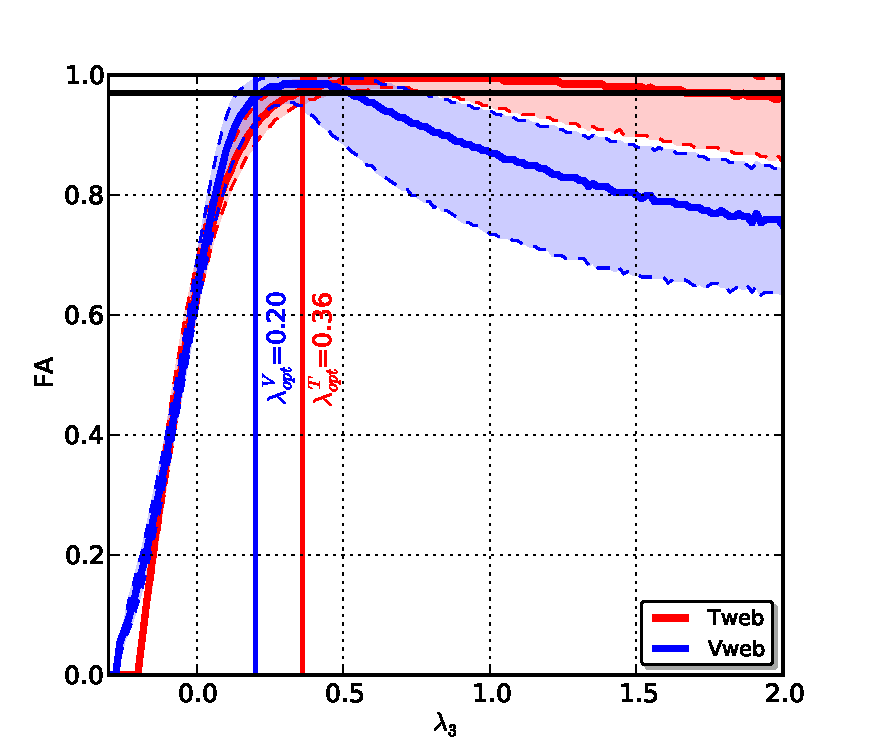
\includegraphics[trim = 2mm 2mm 5mm 10mm, clip, keepaspectratio=true,
  width=0.3\textheight]{./figures/FA_L1.pdf}
  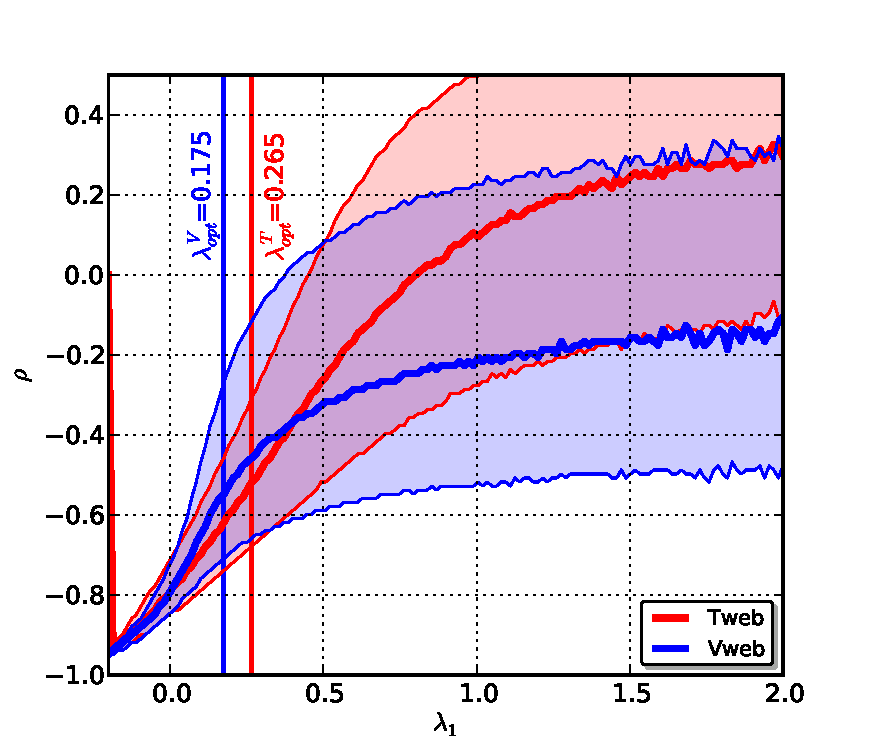
\includegraphics[trim = 2mm 2mm 5mm 10mm, clip, keepaspectratio=true,
  width=0.3\textheight]{./figures/delta_L1.pdf}  
  
  \captionof{figure}{\small In this figure is shown the distribution of the
  fractional anisotropy (left panel) and density field (right panel) with 
  respect to the eigenvalue $\lambda_1$ for each web scheme (T-web, red 
  lines. V-web, blue lines) as calculated over all the cells of the grid.
  Thick central lines correspond to the median of the distribution and 
  coloured regions to the $50\%$ of the cells, delimited by quartiles 
  $Q_1$ and $Q_3$.}

  \label{fig:L1_correlations}
  \vspace{0.1 cm}

\end{figure*}
\end{flushleft}
%.........................................................................



%.........................................................................
%FIGURE 2: Distributions of FA and density regarding the Lambda_1 eigenvalue
\begin{flushleft}
\begin{figure*}
\centering

  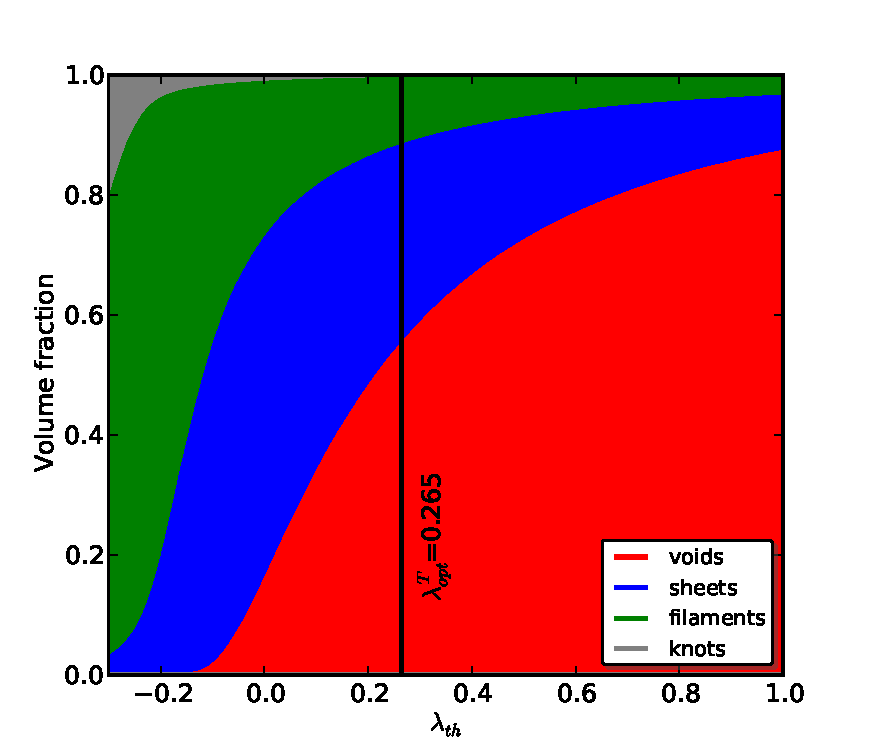
\includegraphics[trim = 2mm 2mm 5mm 10mm, clip, keepaspectratio=true,
  width=0.3\textheight]{./figures/cosmicweb_volume_Tweb.pdf}
  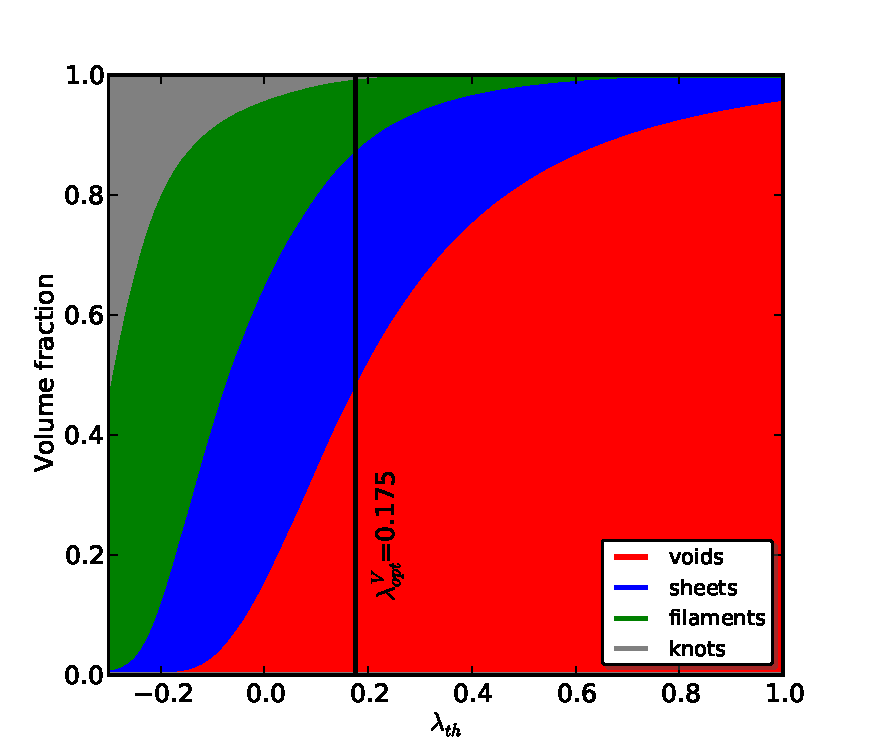
\includegraphics[trim = 2mm 2mm 5mm 10mm, clip, keepaspectratio=true,
  width=0.3\textheight]{./figures/cosmicweb_volume_Vweb.pdf}  
  
  \captionof{figure}{\small In this figure is shown the distribution of the
  fractional anisotropy (left panel) and density field (right panel) with 
  respect to the eigenvalue $\lambda_1$ for each web scheme (T-web, red 
  lines. V-web, blue lines) as calculated over all the cells of the grid.
  Thick central lines correspond to the median of the distribution and 
  coloured regions to the $50\%$ of the cells, delimited by quartiles 
  $Q_1$ and $Q_3$.}

  \label{fig:L1_correlations}
  \vspace{0.1 cm}

\end{figure*}
\end{flushleft}
%.........................................................................


%.........................................................................
%FIGURE 3: Percolation Analysis
\begin{flushleft}
\begin{figure*}
\centering

  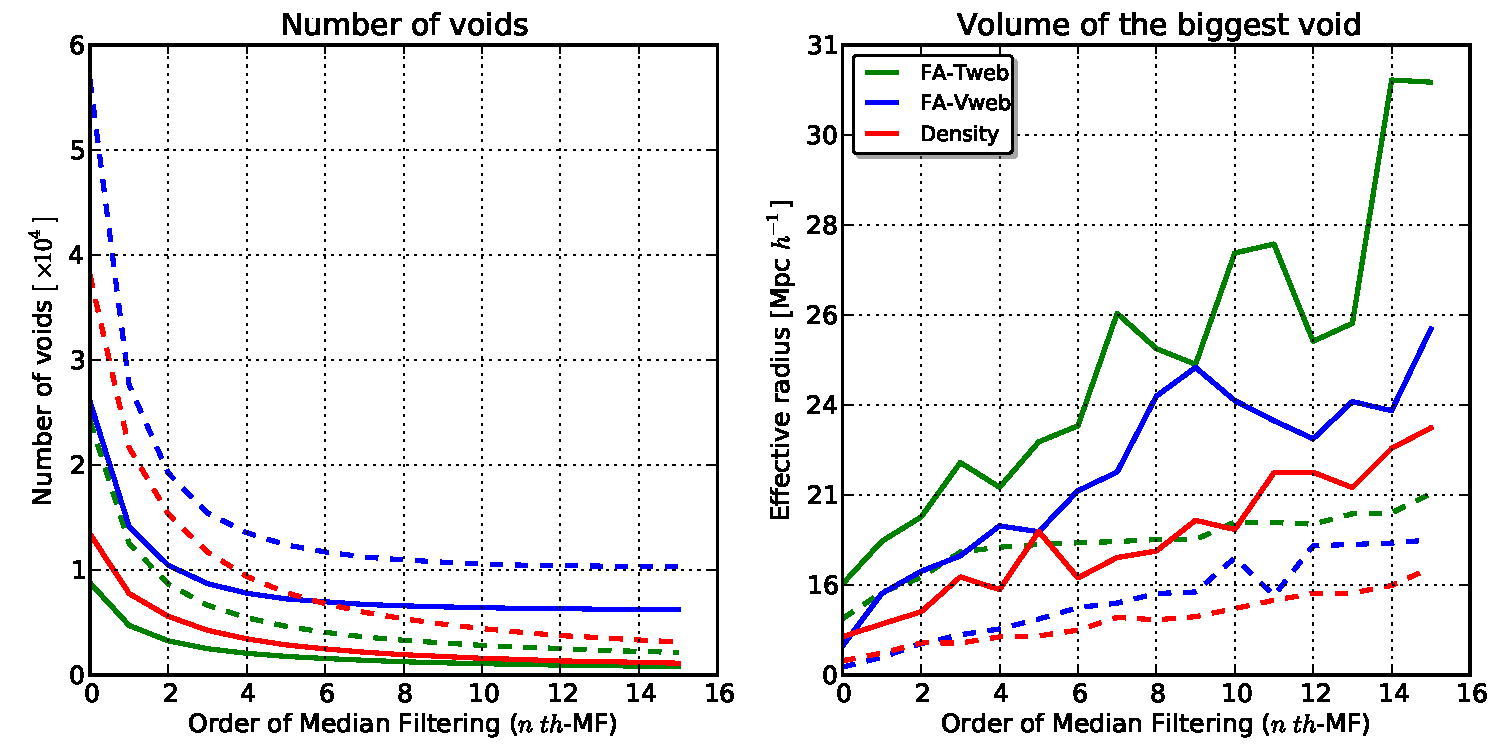
\includegraphics[trim = 0mm 0mm 0mm 0mm, clip, keepaspectratio=true,
  width=0.6\textheight]{./figures/voids_percolation_analysis.pdf}
  
  \captionof{figure}{\small Volume functions of voids catalogued by each 
  used scheme. Left panel (watershed transform over the FA field of the T-web 
  scheme). Central panel (over the FA field of the V-web scheme). Right panel 
  (over the density field). Gray curves correspond to voids without boundary 
  removal whereas black curves are associated to voids merged through boundary 
  removal process. Dotted lines correspond to original continuous fields, 
  while segmented lines correspond to fields with a 1st-order median filtering 
  and continuous lines to a 2nd-order median filtering.}

  \label{fig:FA_field}
  \vspace{0.1 cm}

\end{figure*}
\end{flushleft}
%.........................................................................


%.........................................................................
%FIGURE 4: volume functions
\begin{flushleft}
\begin{figure*}
\centering

  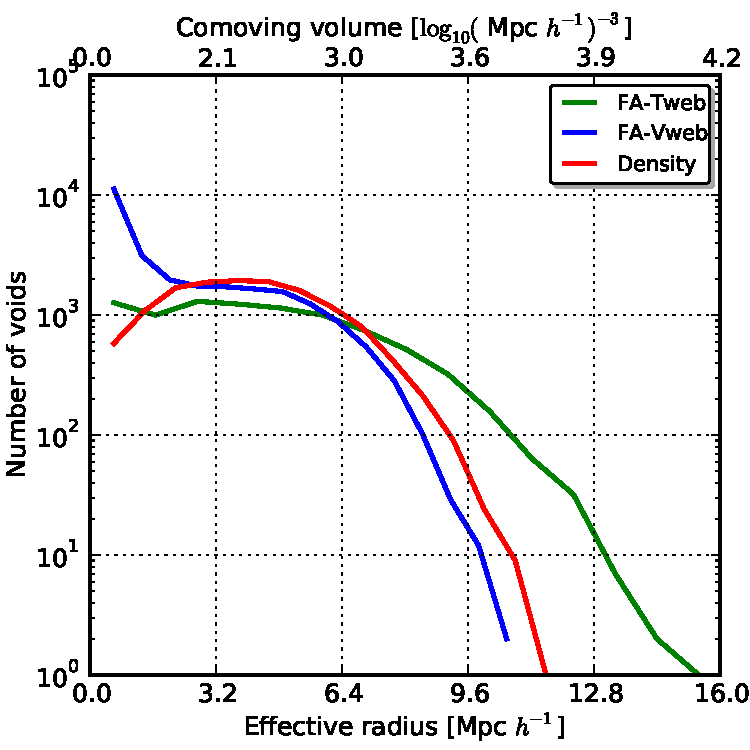
\includegraphics[trim = 0mm 0mm 0mm 0mm, clip, keepaspectratio=true,
  width=0.3\textheight]{./figures/voids_regions_volume_all.pdf}
  
  \captionof{figure}{\small Volume functions of voids catalogued by each 
  used scheme. Left panel (watershed transform over the FA field of the T-web 
  scheme). Central panel (over the FA field of the V-web scheme). Right panel 
  (over the density field). Gray curves correspond to voids without boundary 
  removal whereas black curves are associated to voids merged through boundary 
  removal process. Dotted lines correspond to original continuous fields, 
  while segmented lines correspond to fields with a 1st-order median filtering 
  and continuous lines to a 2nd-order median filtering.}

  \label{fig:FA_field}
  \vspace{0.1 cm}

\end{figure*}
\end{flushleft}
%.........................................................................


%.........................................................................
%FIGURE 5: FA and vissual impression
\begin{flushleft}
\begin{figure*}
\centering

  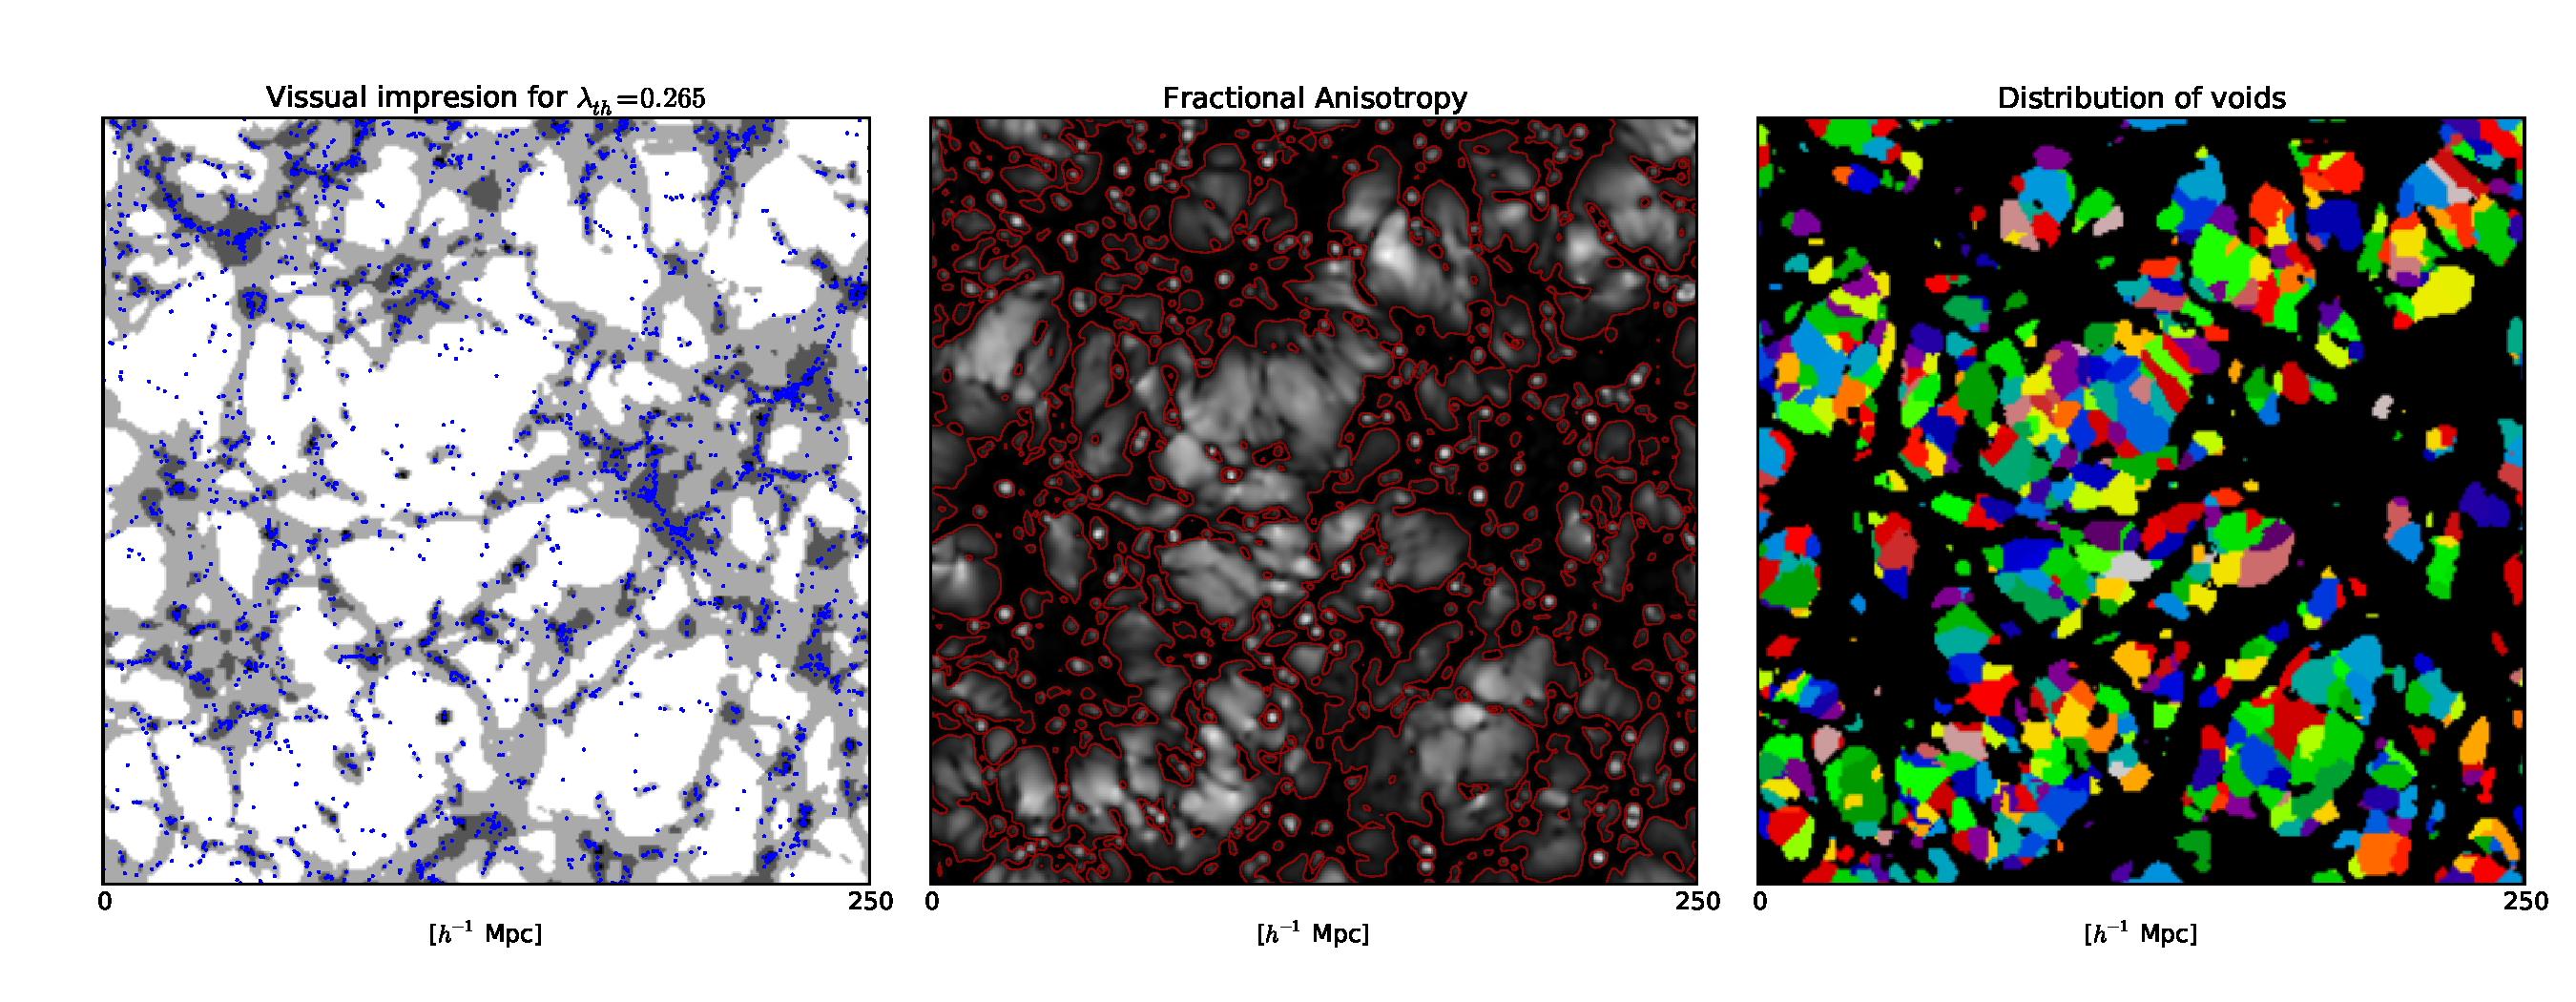
\includegraphics[trim = 16mm 10mm 5mm 12mm, clip, keepaspectratio=true,
  width=0.73\textheight]{./figures/cosmicweb_FA_Tweb.pdf}
  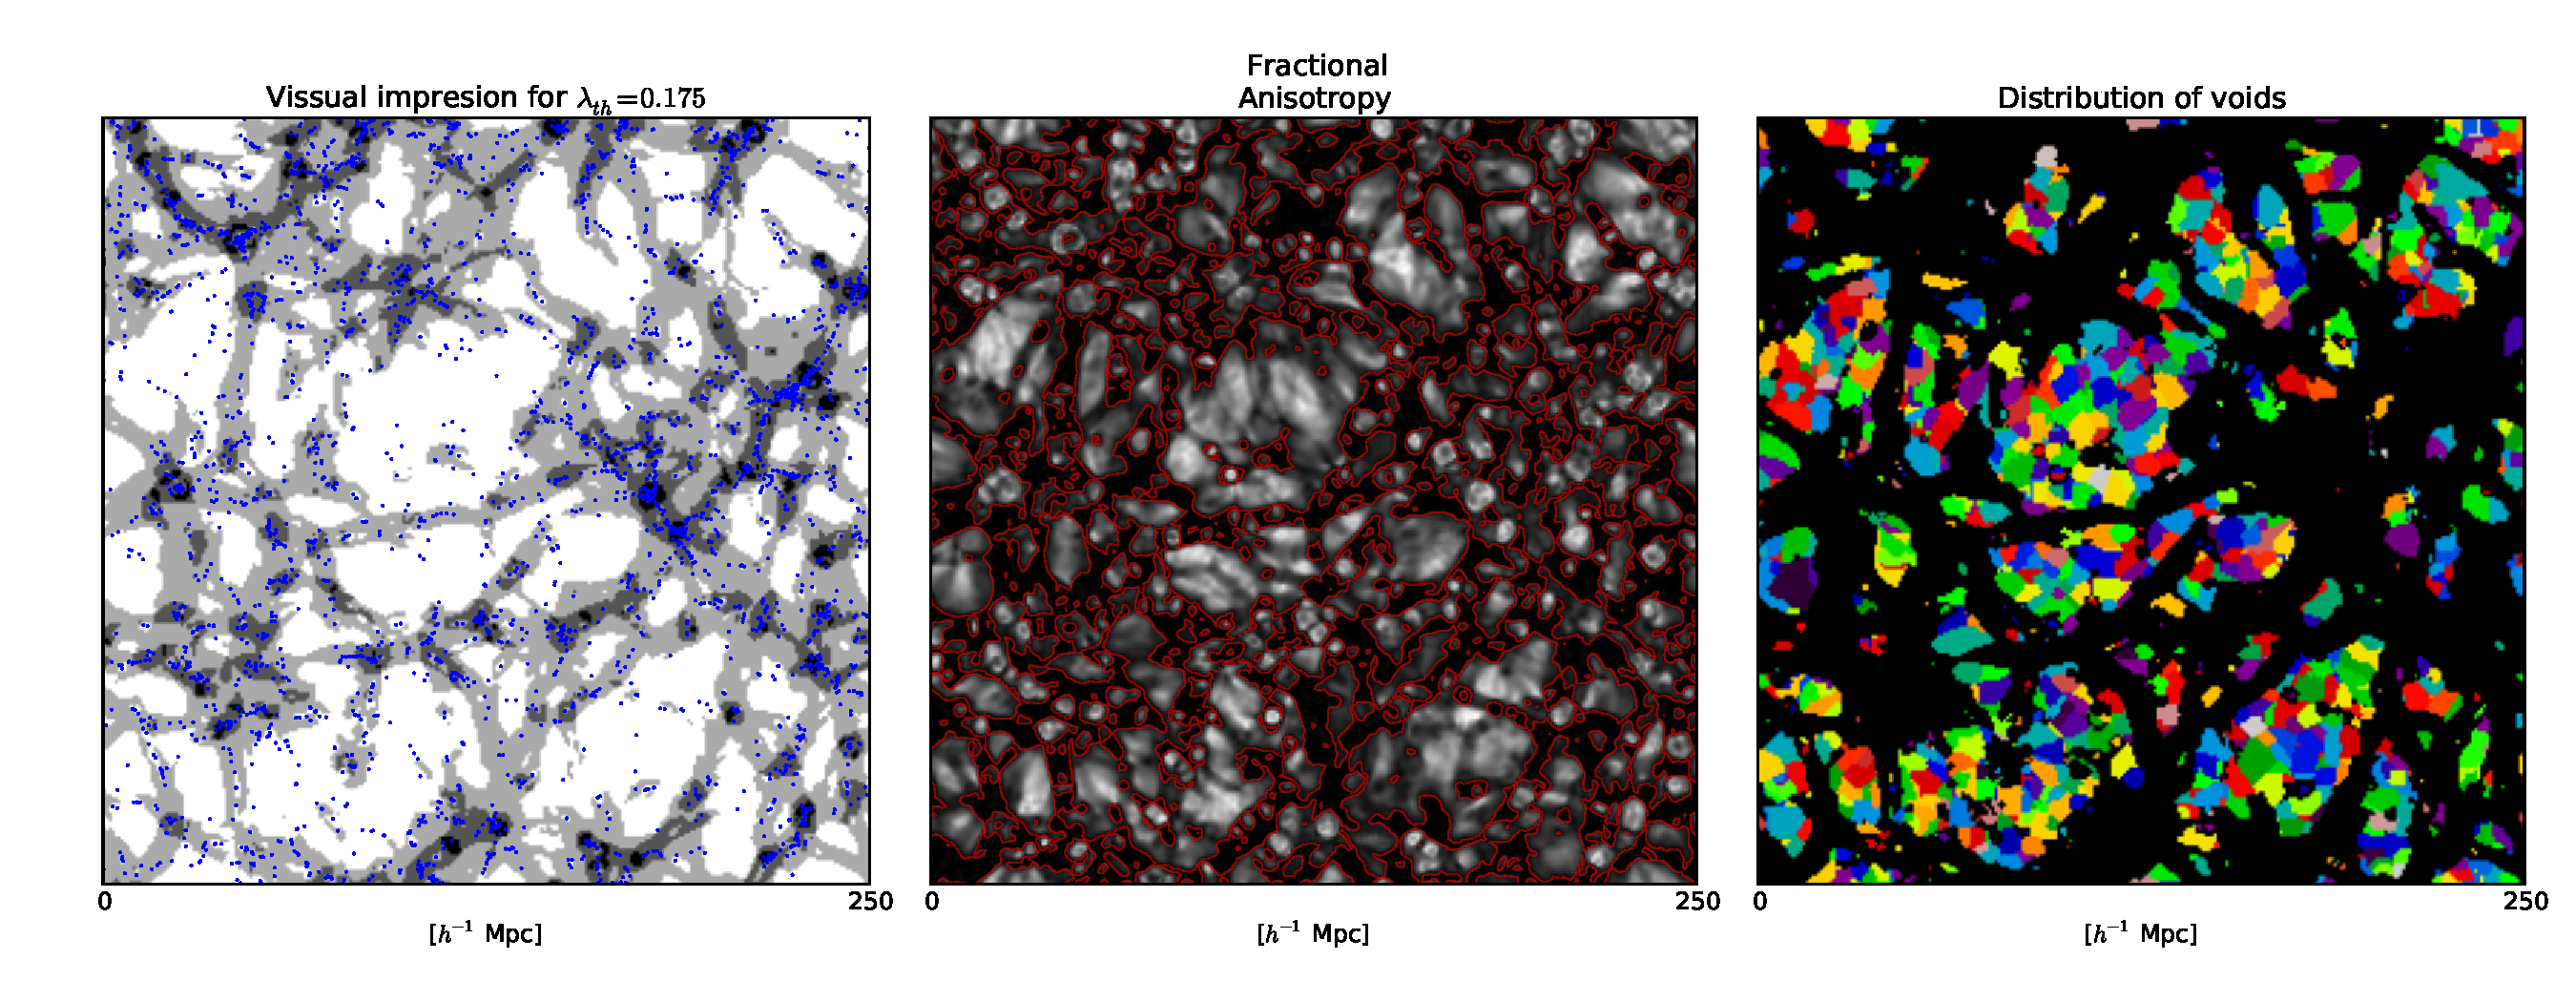
\includegraphics[trim = 16mm 10mm 5mm 12mm, clip, keepaspectratio=true,
  width=0.73\textheight]{./figures/cosmicweb_FA_Vweb.pdf}
  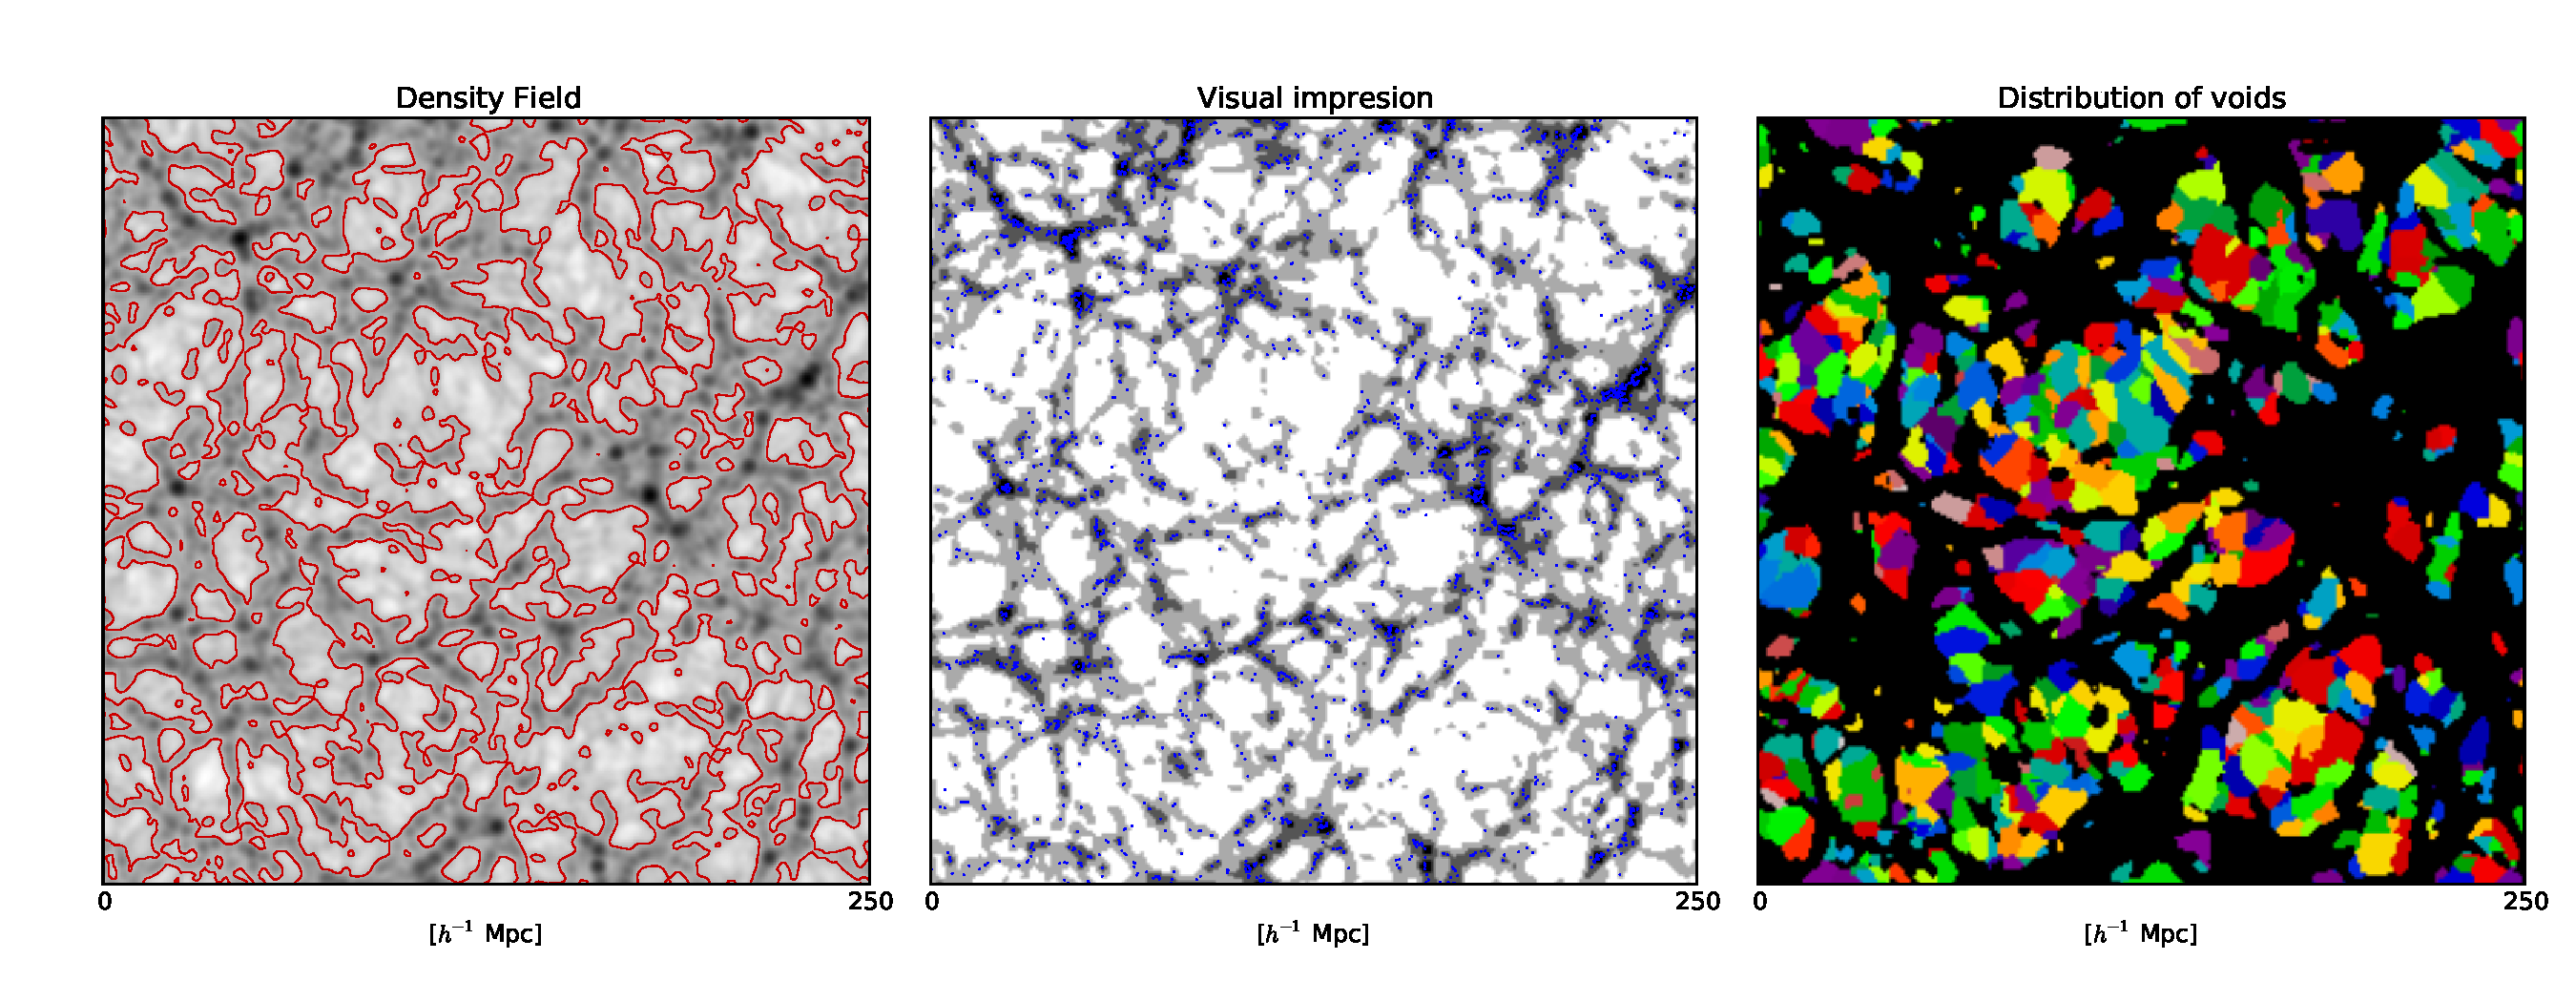
\includegraphics[trim = 16mm 10mm 5mm 12mm, clip, keepaspectratio=true,
  width=0.73\textheight]{./figures/cosmicweb_density.pdf}
  
  \captionof{figure}{\small In left panels is shown the visual impression 
  of the cosmic web for each web scheme (T-web, upper panels. V-web, lower 
  panels) obtained for $\lambda_{th}=0.0$. It can be seen each one of the 
  defined types of environment, where voids corresponds to white zones, 
  sheets to gray, filaments to dark gray and finally knots to black regions. 
  In the right panels is shown the fractional anisotropy field for the same 
  slide of the simulation and for each web schemes, where black regions 
  correspond to FA$=1$ and white regions to FA$=0$. It can be noticed the 
  degeneration of low values of FA for knots and central regions of voids, 
  while high values of FA (FA $\lesssim 1$) are consistent with filaments 
  and highly planar sheets. Thin dark red curves correspond to contours of
  $FA=0.95$, which is approximately the transitional FA between voids and
  other cosmological regions.}

  \label{fig:FA_field}
  \vspace{0.1 cm}

\end{figure*}
\end{flushleft}
%.........................................................................


%.........................................................................
%FIGURE 6: shape-distributions
\begin{flushleft}
\begin{figure*}
\centering

  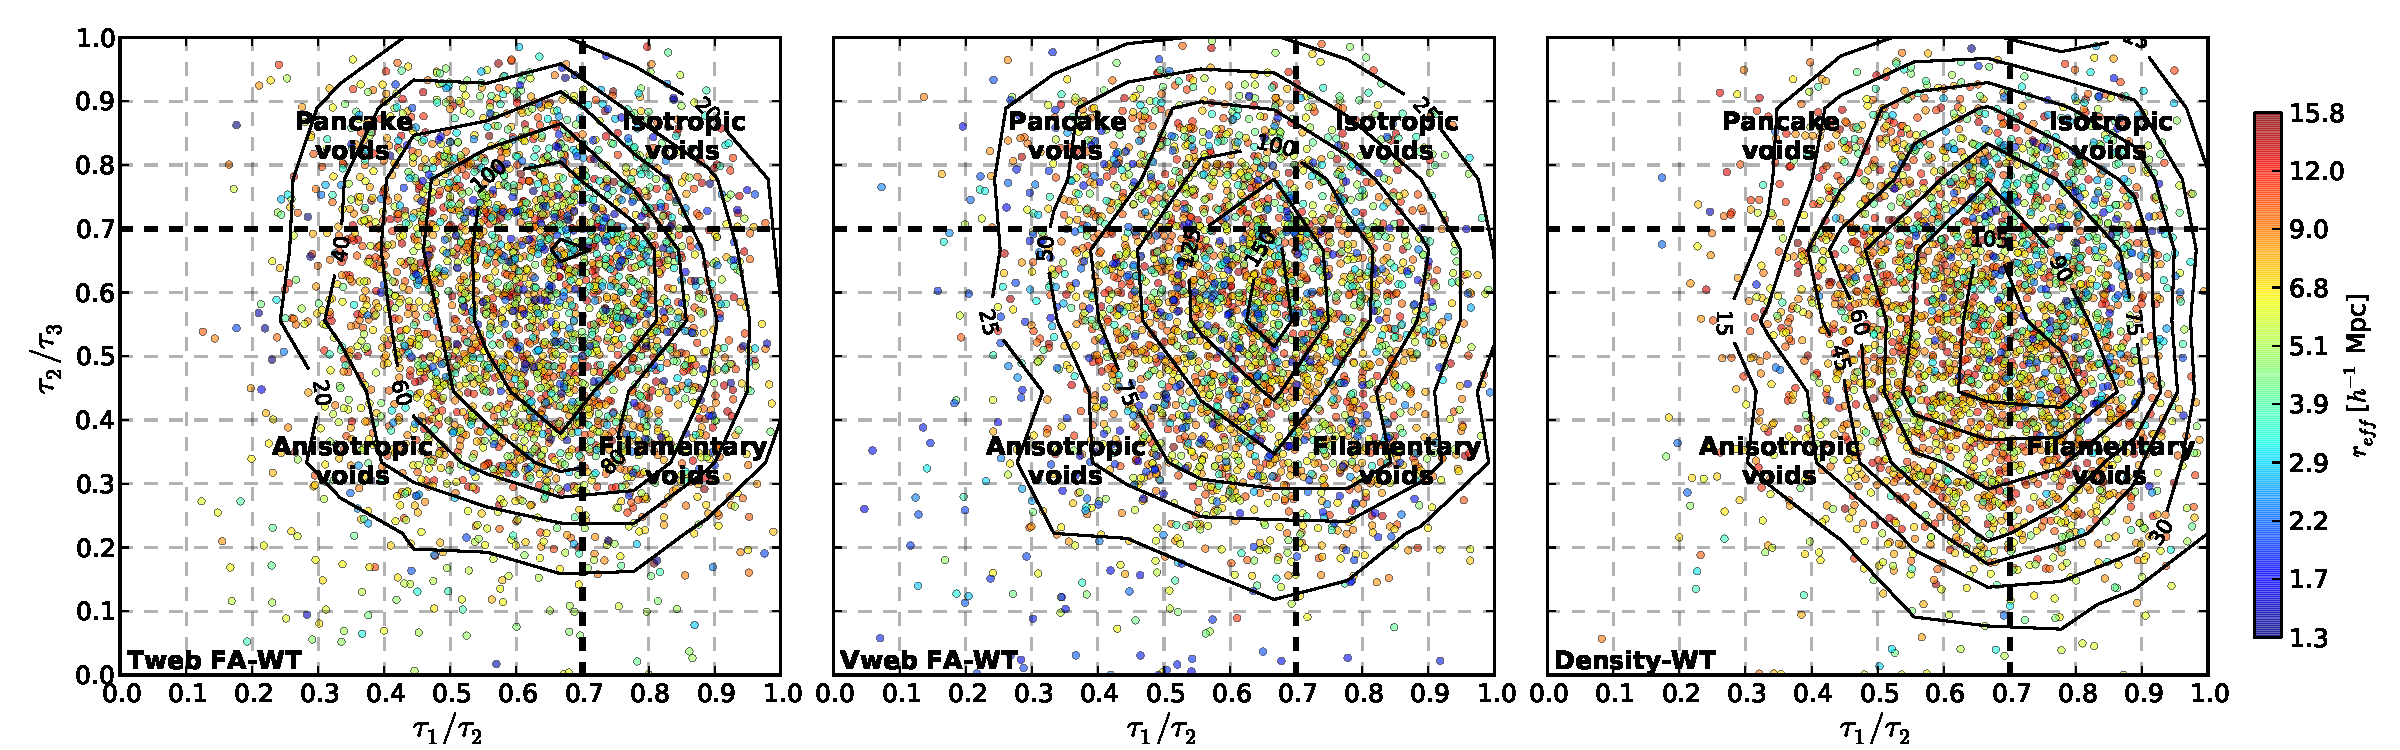
\includegraphics[trim = 6mm 1mm 5mm 4mm, clip, keepaspectratio=true,
  width=0.75\textheight]{./figures/voids_inertia_tensor.pdf}
  
  \captionof{figure}{\small Volume functions of voids catalogued by each 
  used scheme. Left panel (watershed transform over the FA field of the T-web 
  scheme). Central panel (over the FA field of the V-web scheme). Right panel 
  (over the density field). Gray curves correspond to voids without boundary 
  removal whereas black curves are associated to voids merged through boundary 
  removal process. Dotted lines correspond to original continuous fields, 
  while segmented lines correspond to fields with a 1st-order median filtering 
  and continuous lines to a 2nd-order median filtering.}

  \label{fig:FA_field}
  \vspace{0.1 cm}

\end{figure*}
\end{flushleft}
%.........................................................................

\end{document}
